% document
\documentclass[10pt,graphics,aspectratio=169,table]{beamer}
\usepackage{../code}
\usepackage{csquotes}
\usepackage{hyperref}
\usepackage{tikz}
\usepackage{pgfplots}
% theme
\usetikzlibrary{arrows}
\tikzstyle{line}=[draw] % here
\usetikzlibrary{decorations.pathmorphing}
\tikzset{arrow/.style={-latex, shorten >=.5ex, shorten <=.5ex}}

\usetheme{metropolis}
% packages
\title{Lesson 8}
\author{Christian Schwarz, Jakob Krebs}
\date{15.12.2019}
\begin{document}
\maketitle

\begin{frame}{Contents}
    \tableofcontents
\end{frame}

\begin{frame}{Sources and Solutions}
    \begin{itemize}
        \item we publish all code written in this course at \url{https://github.com/jkrbs/c_lessons}
        \item we will publish example solutions of the tasks on same site
        \item send us questions or your solutions to c-lessons@deutschland.gmbh
    \end{itemize}
\end{frame}

\section{Network Protocols}
\subsection{}

\begin{frame}{Osi Reference Model}
    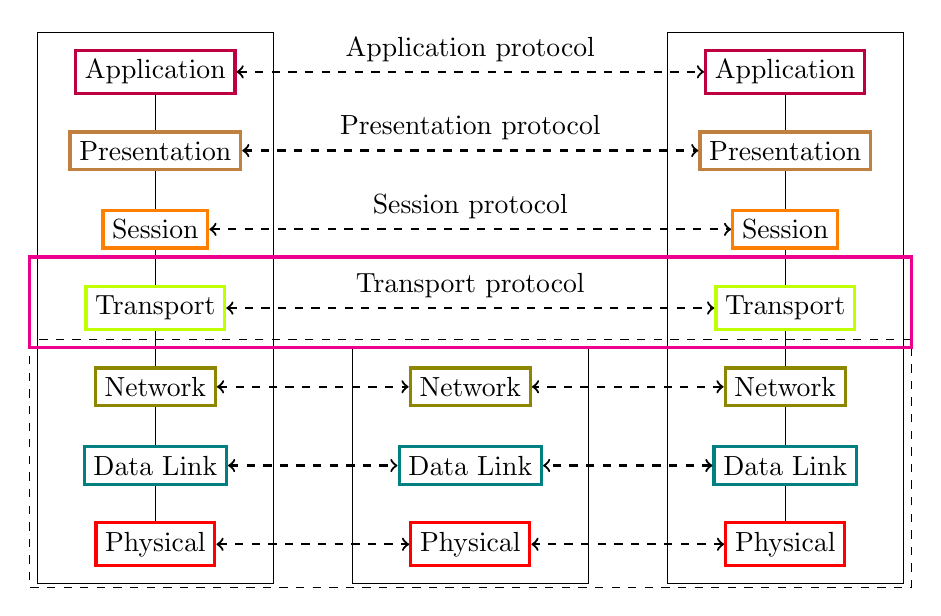
\begin{tikzpicture}[]
        \node [rectangle,draw=purple,very thick](a7) at (0,0) {Application};
        \node [rectangle,draw=brown,very thick](a6) at (0,-1) {Presentation};
        \node [rectangle,draw=orange,very thick](a5) at (0,-2) {Session};
        \node [rectangle,draw=lime,very thick](a4) at (0,-3) {Transport};
        \node [rectangle,draw=olive,very thick](a3) at (0,-4) {Network};
        \node [rectangle,draw=teal,very thick](a2) at (0,-5) {Data Link};
        \node [rectangle,draw=red,very thick](a1) at (0,-6) {Physical};

        \draw (a1) -- (a2);
        \draw (a2) -- (a3);
        \draw (a3) -- (a4);
        \draw (a4) -- (a5);
        \draw (a5) -- (a6);
        \draw (a6) -- (a7);

        \draw (-1.5,.5) rectangle (1.5,-6.5);

        \node [rectangle,draw=purple,very thick](b7) at (8,0) {Application};
        \node [rectangle,draw=brown,very thick](b6) at (8,-1) {Presentation};
        \node [rectangle,draw=orange,very thick](b5) at (8,-2) {Session};
        \node [rectangle,draw=lime,very thick](b4) at (8,-3) {Transport};
        \node [rectangle,draw=olive,very thick](b3) at (8,-4) {Network};
        \node [rectangle,draw=teal,very thick](b2) at (8,-5) {Data Link};
        \node [rectangle,draw=red,very thick](b1) at (8,-6) {Physical};

        \draw (b1) -- (b2);
        \draw (b2) -- (b3);
        \draw (b3) -- (b4);
        \draw (b4) -- (b5);
        \draw (b5) -- (b6);
        \draw (b6) -- (b7);

        \draw (6.5,.5) rectangle (9.5,-6.5);


        \node [rectangle,draw=olive,very thick](c3) at (4,-4) {Network};
        \node [rectangle,draw=teal,very thick](c2) at (4,-5) {Data Link};
        \node [rectangle,draw=red,very thick](c1) at (4,-6) {Physical};

        \draw (2.5,-3.5) rectangle (5.5,-6.5);

        \draw [dashed] (-1.6,-3.4) rectangle (9.6,-6.55);

        \draw [dashed,<->,thick] (a1) -- (c1);
        \draw [dashed,<->,thick] (a2) -- (c2);
        \draw [dashed,<->,thick] (a3) -- (c3);

        \draw [dashed,<->,thick] (b1) -- (c1);
        \draw [dashed,<->,thick] (b2) -- (c2);
        \draw [dashed,<->,thick] (b3) -- (c3);


        \draw [dashed,<->,thick] (a4) -- node [above,midway]{Transport protocol} (b4);
        \draw [dashed,<->,thick] (a5) -- node [above,midway]{Session protocol} (b5);
        \draw [dashed,<->,thick] (a6) -- node [above,midway]{Presentation protocol} (b6);
        \draw [dashed,<->,thick] (a7) -- node [above,midway]{Application protocol} (b7);

        \uncover<2->{
            \draw [magenta, very thick] (-1.6,-2.35) rectangle (9.6,-3.5);
        }
    \end{tikzpicture}
\end{frame}

\begin{frame}{Transport Protocols}
    TCP:
    \begin{itemize}
        \item connection-oriented
        \item three-way-handshake
        \item dialog between two sides
        \item guaranteed data delivery in the same order as sent
    \end{itemize}
    \bigskip
    UDP:
    \begin{itemize}
        \item connectionless
    	\item faster, since it is "best effort" (no error recovery)
		\item no guarantee for sent packages to arrive    	
    \end{itemize}
    % vielleicht auch keine zwei itemize, sondern was schöneres
\end{frame}

\section{Socket Programming}
\subsection{}

\begin{frame}[fragile]{Sockets}
    Sockets are abstractions for connection endpoints to be used by processes.
    Both the server and the client process have a socket which they use to
    send data to each other.\\
    \bigskip
    Sockets are platform-dependend, but the system call interface is similar:
    \begin{description}
        \item[Unix] file descriptors (\lstinline{int})
        \item[Windows] handles for kernel objects
            (\lstinline[morekeywords={*,SOCKET}]{SOCKET})
    \end{description}
    \bigskip
    You will also have to include different headers:
    \begin{lstlisting}[numbers=none]
// Unix
#include <sys/socket.h>
// Windows
#include <windows.h>
\end{lstlisting}
\end{frame}

\begin{frame}[fragile]{\texttt{socket()}}
	Create an endpoint for communication.
	\begin{lstlisting}[numbers=none,morekeywords={*,SOCKET,socklen_t,sockaddr}]
//Unix
int socket(int domain, int type, int protocol);
//windows
SOCKET socket(int domain, int type, int protocol);
\end{lstlisting}
	\begin{description}
		\item [domain] Communication domain for the socket \\
            {\verb+[AF_INET, AF_INET6, os-specific domains]+}
		\item [type] Type of the socket \\
            {\verb+[SOCK_STREAM, SOCK_DGRAM, SOCK_RAW, ...]+}
		\item [protocol] The protocol to be used \\
            {\verb+[0, IPPROTO_TCP, IPPROTO_UDP, ...]+}
		\item [return value] File descriptor / socket handle if successful, -1
            otherwise
	\end{description}
\end{frame}
% -- hier evtl. noch ein Frame mit Erklärung der Netzwerkadressrechnung


% - close[socket]()
\begin{frame}[fragile]{\texttt{close[socket]()}}
Close an existing socket / file descriptor.
	\begin{lstlisting}[numbers=none,morekeywords={*,SOCKET,socklen_t,sockaddr}]
//Unix
int close(int fildes);
//windows
int closesocket(SOCKET socket);
\end{lstlisting}
	\begin{description}
		\item [fildes/socket] File descriptor / handle of the socket to close
		\item [return value] Exit status (0 = success, -1 = failure)
	\end{description}
	\bigskip
	Do not leak file descriptors!
\end{frame}

\begin{frame}[fragile]{\texttt{connect()}}
    Connect a socket to another via the network.
    \begin{lstlisting}[numbers=none,morekeywords={*,SOCKET,socklen_t,sockaddr}]
// Unix
int connect(int socket, const struct sockaddr *address,
            socklen_t address_len);
// Windows
int connect(SOCKET socket, const struct sockaddr *address,
            int address_len);
\end{lstlisting}
    \begin{description}
        \item[socket] Socket to be connected
        \item[address] Structure containing target IP address and port
        \item[address\_len] Size of \texttt{*address} in memory
        \item[return value] Exit status (0 = success, -1 = failure)
    \end{description}
    \bigskip
    UDP sockets don't establish a connection $\rightarrow$ \texttt{connect()} is
    optional.
\end{frame}

\begin{frame}[fragile]{\texttt{bind()}}
    Bind an address to a socket.
    \begin{lstlisting}[numbers=none,morekeywords={*,SOCKET,socklen_t,sockaddr}]
// Unix
int bind(int socket, const struct sockaddr *address,
         socklen_t address_len);
// Windows
int bind(SOCKET socket, const struct sockaddr *address,
         int address_len);
\end{lstlisting}
    \begin{description}
        \item[socket] Socket to be bound
        \item[address] Structure containing IP address and port
        \item[address\_len] Size of \texttt{*address} in memory
        \item[return value] Exit status (0 = success, -1 = failure)
    \end{description}
    \bigskip
    Naming a socket is necessary for connections from the outside!
\end{frame}

\begin{frame}[fragile]{\texttt{listen()}}
    Enable listening for connections to a specific socket.
    \begin{lstlisting}[numbers=none,morekeywords={*,SOCKET}]
// Unix
int listen(int socket, int backlog);
// Windows
int listen(SOCKET socket, int backlog);
\end{lstlisting}
    \begin{description}
        \item[socket] Socket to put into listening mode
        \item[backlog] Hint for an upper bound of the number of outstanding
            connections in the listening queue of the socket
        \item[return value] Exit status (0 = success, -1 = failure)
    \end{description}
    \bigskip
    Calling \texttt{listen()} on a socket is necessary to accept incoming TCP
    connections on a server.
\end{frame}

\begin{frame}[fragile]{\texttt{accept()}}
    Accept a new connection on a socket.
    \begin{lstlisting}[numbers=none,morekeywords={*,SOCKET,sockaddr,socklen_t}]
// Unix
int accept(int socket, struct sockaddr *restrict address,
           socklen_t *restrict address_len);
// Windows
SOCKET accept(SOCKET socket, struct sockaddr *address,
              int *address_len);
\end{lstlisting}
    \begin{description}
        \item[socket] Listening socket
        \item[address] Where to store the address of the
            connecting socket
        \item[address\_len] Size of \texttt{*address} in memory
        \item[return value] Socket for the new connection on success, invalid
            descriptor otherwise
    \end{description}
    \bigskip
    By default, \texttt{accept()} blocks if the socket's connection queue is empty!
\end{frame}

% - send()
\begin{frame}[fragile]{\texttt{send[to]()}}
    Send a message on a socket.
    \begin{lstlisting}[numbers=none,morekeywords={*,SOCKET,sockaddr,socklen_t,size_t}]
// Unix
int send[to](int socket, const void *buffer, size_t length,
		 	 int flags[, const struct sockaddr *dest_addr,
    	 	 socklen_t dest_len]);
// Windows
int send[to](SOCKET socket, const char *buffer, int lenght,
             int flags[, const struct sockaddr *dest_addr,
             int dest_len]);
\end{lstlisting}
    \begin{description}
        \item[socket] Socket to send from
        \item[buffer] Pointer to the message to be transmitted
        \item[length] Length of the message
        \item[flags] Type of transmission
        \item[dest\_addr] Optional target socket
        \item[dest\_len] Size of \texttt{*dest\_addr} in memory
        \item[return value] Number of bytes sent or -1 on error
    \end{description}
\end{frame}

% recv()
\begin{frame}[fragile]{\texttt{recv[from]()}}
    Recieve a message on a socket.
    \begin{lstlisting}[numbers=none,basicstyle=\scriptsize,morekeywords={*,SOCKET,sockaddr,socklen_t}]
// Unix
int recv[from](int socket, const void *buffer, size_t length,
               int flags[, struct sockaddr *restrict address,
		 	   socklen_t *restrict address_len]);
// Windows
int recv[from](SOCKET socket, const char *buffer, int length,
		       int flags[, struct sockaddr *address,
               int *address_len]);
\end{lstlisting}
    \begin{description}
        \item[socket] The connected socket
        \item[buffer] Pointer where to put the recieved message
        \item[length] Length of the message buffer
        \item[flags] Type of transmission
        \item[adress] Optional sending socket
        \item[adress\_len] Size of \texttt{*adress} in memory
        \item[return value] \verb+#+bytes recieved, 0 (connection closed), or
            -1 (failure)
    \end{description}
    \bigskip
    
\end{frame}

\section{Task}
\begin{frame}[fragile]{a simple server}
let's write a program which listens on port \code{1337} and prints the send packet payload.

the output should be like this:
\begin{codeblock}
[sender address]: [message]
23.42.23.42: lame course :p
\end{codeblock}
\end{frame}
\begin{frame}{send us your name}
send us your name on a tcp connection to \code{dvorak.krbs.me(IPv4 Address: 116.203.113.16)} on port \code{1337}

What you send us, will be printed on the the beamer.

have a try. Our program from the last task will run there.
\end{frame}
\end{document}
